\section{Method}
\label{sec:method}

The method keeps a set of competing physical explanations for an observed image,
predicts what each implies after a candidate camera motion, measures how far those
predictions diverge, and answers only when some available motion is guaranteed to
separate every explanation still in contention.

\begin{figure}[t]
\begin{center}
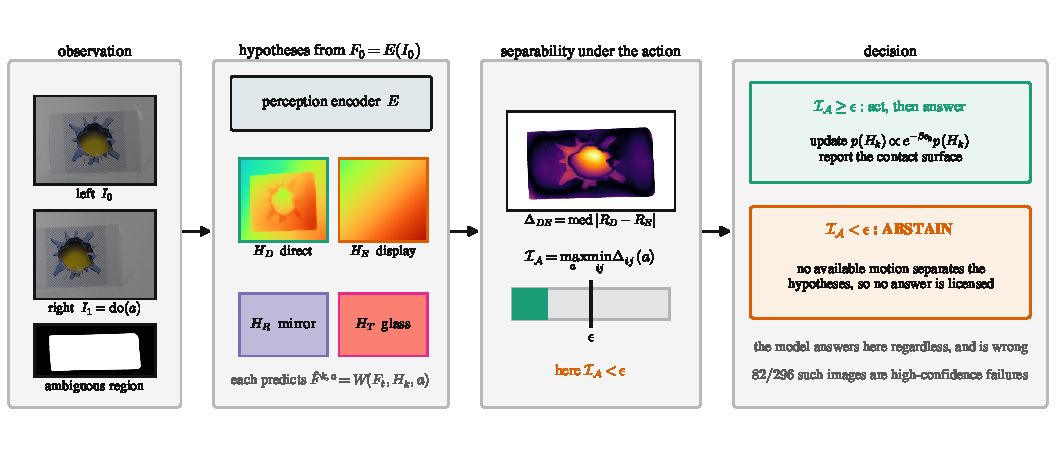
\includegraphics[width=\linewidth]{figures/fig_system.pdf}
\end{center}
\caption{\textbf{The method on one real image.} A stereo pair supplies an executed
action, and the annotated region marks where the surface is ambiguous. The
encoder's geometry gives $H_D$ directly and, fitted to a plane over the same
region, $H_E$; mirror and glass enter the same way where the scene admits them.
Warping the second view under each hypothesis gives the separability $\Delta_{DE}$
of \eqref{eq:delta-photometric}, and identifiability \eqref{eq:identifiability} is
compared against the perceptual threshold. It lies below it, so
\eqref{eq:abstain} correctly declines to answer on a scene no available motion
resolves, while the predictor answers and is wrong.
Depth maps are from a published checkpoint used as released.}
\label{fig:system}
\end{figure}

\subsection{Hypotheses and the action set}
\label{sec:formulation}

Let $I_0$ be an image at reference pose $C_0$ and $F_0 = E(I_0)$ the geometry a
perception encoder $E$ reports for it, as landmarks carrying image coordinates,
depths and visibility flags. Rather than returning $F_0$ alone, a family of
image-formation hypotheses is kept: $H_D$ asserts the structure is physically
present, $H_E$ that it is depicted on a flat emissive panel, $H_R$ that it is a
virtual image in a planar mirror, and $H_T$ that it is seen through a planar
transparent slab. Each places the first touchable surface elsewhere, which is the
distinction a contact-based cost makes. They are matched by construction, being
pixel-identical at $C_0$, so any later gain from moving the camera is attributable
to the motion rather than to a residual appearance difference.

The observer acts. An action $a \in SE(3)$ is a rigid camera motion applied as an
explicit intervention,
\begin{equation}
\label{eq:intervention}
\mathrm{do}\!\left(C_1 = C_0 \cdot a\right),
\end{equation}
where $C_0$ is the reference pose, $C_1$ the resulting pose and $\cdot$ composition
of rigid transforms. The $\mathrm{do}(\cdot)$ notation replaces conditioning
because the viewpoint is chosen rather than encountered, so the evidence is
attributable to the action. Actions come from a bounded, enumerable set $\mathcal{A}$: translations of
$\{0.05, 0.10, 0.20, 0.30\}$~m along three axes and rotations of
$\{5^\circ, 10^\circ\}$ in yaw and pitch, both directions, plus the null action,
giving $|\mathcal{A}| = 33$ under a budget of $0.35$~m and $15^\circ$. The budget is
modest because the setting is a device making a small corrective movement rather
than one repositioning freely. Finiteness lets identifiability be evaluated by
enumeration before any motion, which is what makes abstention possible in advance
of acting. Landmarks are the encoder's own output sampled on a fixed grid over the
scene, each carrying an image coordinate, a depth and a visibility flag; visibility
under a hypothesis is decided by z-buffering that hypothesis' predicted geometry,
so a landmark occluded under one mechanism and not another contributes to
$D_{\text{occlusion}}$.

\subsection{Predicting the consequence of an action}
\label{sec:transition}

Each hypothesis maps current geometry and a candidate action to a predicted
observation,
\begin{equation}
\label{eq:transition}
\hat{F}^{\,k,a} \;=\; W\!\left(F_t,\, H_k,\, a\right),
\end{equation}
where $F_t$ is the geometry at time $t$, $H_k$ the $k$-th hypothesis, $a$ the
candidate action and $\hat{F}^{\,k,a}$ what $H_k$ predicts after executing $a$. The
transition $W$ applies one shared projection to every hypothesis and differs only
in the world each asserts: a panel paints content on the screen plane, gaining no
differential parallax; a mirror keeps the parallax of virtual structure while
adding moving virtual images of observer-attached markers; a slab displaces content
axially. Sharing the projection makes any difference between predictions
attributable to the mechanism rather than to rendering.

The mechanisms are planar for a reason the construction depends on. A planar
mirror reflects exactly across a plane and a planar slab displaces content
axially by $d\,(1 - 1/n)$, so each transition is closed form. That is what makes the counterfactuals \emph{matched}: reference views can be
made pixel-identical to numerical precision, and any divergence after an action
is attributable to the mechanism rather than to approximation error. A curved
surface admits no exact transition, and a learned one would reintroduce the
confound the shared projection removes. The restriction is a condition for the
experiment to be clean rather than a limit of the formalism, which is
independent of it (Appendix~\ref{sec:supp-extension}).

\subsection{Separability, identifiability and abstention}
\label{sec:separability}

Pairwise separability is the distance between the consequences two hypotheses
predict for the same action,
\begin{equation}
\label{eq:separability}
\Delta_{ij}(a) \;=\; D\!\left(\hat{F}^{\,i,a},\, \hat{F}^{\,j,a}\right),
\end{equation}
where $i,j$ index two hypotheses and $D$ is a composite distance,
\begin{equation}
\label{eq:distance}
D \;=\; \lambda_m D_{\text{motion}} + \lambda_o D_{\text{occlusion}}
      + \lambda_g D_{\text{geometry}} + \lambda_f D_{\text{feature}} .
\end{equation}
Here $D_{\text{motion}}$ is the root-mean-square image-space displacement between
the two predicted landmark sets over jointly visible landmarks, in pixels;
$D_{\text{occlusion}}$ counts landmarks whose predicted visibility differs;
$D_{\text{geometry}}$ is the root-mean-square 3-D distance between back-projected
landmarks; $D_{\text{feature}}$ is reserved for a learned feature distance; and
$\lambda_m, \lambda_o, \lambda_g, \lambda_f$ weight them. Throughout
$\lambda_m = 1$, $\lambda_o = 4.0$~px per disagreeing landmark, and
$\lambda_g = \lambda_f = 0$, placing $D$ in pixels so the threshold below is a
perceptual displacement threshold in the same units. The occlusion term counts
rather than takes a fraction, since a fraction would be diluted by the landmark
count; its weight places one unambiguous appearance or disappearance clearly above
the $1$~px threshold, which matters because that is frequently the only cue a
mirror offers. Priors over hypotheses are uniform at $t = 0$. The sensitivity of
the decision to $\epsilon$ and to the admissibility criterion is reported in
Appendix~\ref{sec:supp-sensitivity}.

The quantity of interest is the best separability the action set attains,
\begin{equation}
\label{eq:identifiability}
\mathcal{I}_{\mathcal{A}}\!\left(H_i, H_j\right)
\;=\; \max_{a \in \mathcal{A}} \; \Delta_{ij}(a),
\end{equation}
so a pair counts as separable if any single permitted motion would distinguish it.
The system abstains when
\begin{equation}
\label{eq:abstain}
\min_{(i,j)} \; \mathcal{I}_{\mathcal{A}}\!\left(H_i, H_j\right) \;<\; \epsilon ,
\end{equation}
the minimum running over pairs still in contention. The order matters: a maximum
over actions inside a minimum over pairs licenses an answer only if some action
separates every undecided pair, since the pair left unseparated is exactly where an
error would be made. The threshold is fixed at $\epsilon = 1.0$~px and not tuned,
being a property of the sensor and the perceptual criterion: altering it changes
what ``identifiable'' denotes and relabels the benchmark rather than improving
performance on it.

\subsection{Choosing the intervention}
\label{sec:selection}

Two objectives are compared. The first is the summed objective standard in active
perception,
\begin{equation}
\label{eq:sum}
a^{\star}_{\text{sum}} \;=\; \arg\max_{a \in \mathcal{A}}
\;\sum_{i<j} p_i\, p_j\, \Delta_{ij}(a),
\end{equation}
where $p_i, p_j$ are posterior probabilities, so still-plausible pairs contribute
more. Such a sum can be maximised by an action separating pairs not in contention
while leaving the deciding pair unseparated, since a large term compensates for a
zero one. The second replaces the sum with the weakest contending pair,
\begin{equation}
\label{eq:maximin}
a^{\star}_{\text{maximin}} \;=\; \arg\max_{a \in \mathcal{A}}
\;\min_{(i,j) \in \mathcal{C}} \; w_{ij}\, \Delta_{ij}(a),
\end{equation}
where $\mathcal{C}$ collects pairs whose joint posterior mass has not collapsed and
$w_{ij}$ weights each by that mass. The form follows from the abstention rule: a
decision needs every contending pair separated, so the binding quantity is the
smallest separability rather than the sum. This is $T$-optimality from optimal
design for model discrimination
\citep{atkinson1975design,hunter1965experimental}, applied to active vision.

\paragraph{Which quantity is available, and when.}
Both objectives are stated over hypothesis \emph{pairs} and so need at least two
pairs to differ. Four mechanisms give six pairs in the synthetic benchmark, where
the weakest-pair form is the operative criterion. A calibrated stereo pair supports
two mechanisms and hence one pair, so on real photographs \eqref{eq:sum} and
\eqref{eq:maximin} coincide. Selection there runs instead through the belief update
of \eqref{eq:belief}: among viewpoints the observer could occupy, prefer the one at
which some hypothesis best accounts for the view actually obtained,
\begin{equation}
\label{eq:evidence-selection}
a^{\star}_{\text{evidence}} \;=\; \arg\min_{a \in \mathcal{A}} \;
\min_{k} \; e_k(a),
\end{equation}
with $e_k(a)$ the residual of hypothesis $k$ after executing $a$. Both rules act on
the same belief machinery, one through the separability entering it and one through
the residual leaving it, and each is used where the evidence it needs exists.

\subsection{Belief update and output}
\label{sec:belief}

After the selected action is executed and $O'$ observed, each hypothesis has
residual $e_k = D(\hat{F}^{\,k,a^\star}, E(O'))$ under the same
distance~\eqref{eq:distance}, so prediction error and separability share a scale.
Belief updates multiplicatively,
\begin{equation}
\label{eq:belief}
p_{t+1}(H_k) \;\propto\; \exp\!\left(-\beta\, e_k\right)\, p_t(H_k),
\end{equation}
where $p_t(H_k)$ is the prior mass on hypothesis $k$, $e_k$ its residual in pixels
and $\beta$ converts error into log-likelihood; $\beta = 1.0$ makes a one-pixel
error cost one nat. A posterior floor stops one unlucky observation eliminating a
hypothesis permanently. The system then names the mechanism and reports its contact
geometry, the first physical surface along each ray, which is the glass for a
mirror and the panel for a display. Commitment is withheld when the posterior
maximum does not exceed $\tau = 0.45$, set just below the $0.5$ tie a forced choice
over a two-way ambiguity produces, so such a choice counts as false certainty
rather than caution.

\subsection{Benchmark and metrics}
\label{sec:benchmark}

Each base scene is instantiated under every mechanism with content adjusted so the
reference views coincide, to a maximum deviation of order $10^{-14}$~px, making
chance-level single-view performance a verified property rather than an assumption.
Configurations no permitted action resolves, namely view-tracked displays within
their aperture and mirrors mimicking an opening, are included deliberately: without
them a method that never abstains would be indistinguishable from one that abstains
correctly. Splits are formed by base scene.

Four quantities are reported. Causal explanation accuracy (CEA) is
$P(\hat{H} = H^\star)$ with abstention counted as an error, and committed accuracy
is $P(\hat{H} = H^\star \mid \text{answered})$; the first penalises caution and the
second rewards it, so together they expose the trade between answering and being
right. False physical certainty (FPCR) is
$P(\max_k p(H_k) > \tau \mid y_{\mathrm{id}} = 0)$, measured only on unresolvable
cases, and is what abstention exists to reduce. Normalised regret compares the
chosen action's utility against the best available.

\subsection{Protocol for real photographs}
\label{sec:real-protocol}

A calibrated rectified stereo pair supplies one executed action with known
parameters, the baseline translation, so real data is the case $|\mathcal{A}| = 1$.
Four elements stop the measurement absorbing the effect under study.

\textbf{Calibration outside, scoring inside.} A monocular predictor returns
relative inverse depth, defined up to unknown scale $s$ and shift $t$, fitted by
least squares against reference disparity on the non-ambiguous region and applied
inside it, giving the disparity predicted under $H_D$,
\begin{equation}
\label{eq:align}
d_{D} \;=\; s\,\hat{p} + t ,
\end{equation}
with $\hat{p}$ the raw prediction. Determining the two parameters where the
predictor performs well stops them absorbing the discrepancy under study. The
disparity under $H_E$ is the least-squares plane through $d_D$ over that region,
fitted to the prediction and never the reference, which would place ground truth
inside a quantity that must be computable at test time.

\textbf{Separability is measured photometrically.} The right image is warped into
the left frame under each hypothesis, using the rectified-stereo relation that
column $x$ with disparity $d$ corresponds to column $x - d$ in the other view,
\begin{equation}
\label{eq:warp}
R_{k}(x, y) \;=\; I_{\text{right}}\!\left(x - d_{k}(x,y),\; y\right),
\qquad k \in \{D, E\},
\end{equation}
and separability is the median absolute difference between the two warps inside the
region,
\begin{equation}
\label{eq:delta-photometric}
\Delta_{DE} \;=\; \operatorname{median}\left|R_{D} - R_{E}\right| .
\end{equation}
Both terms warp the same photograph, so illumination, sensor noise and
rectification error appear in both and cancel. Intensity units are deliberate: a
disparity disagreement is visible only where the image carries structure to reveal
it, so on a featureless region two hypotheses predict different geometry and
identical pixels, and the scene is unidentifiable at any baseline.

\textbf{Ground truth is admitted only when it can arbitrate.} A printed sheet or
panel is flat, so reference disparity inside the region should be planar. Where it
is not, stereo matching has locked onto displayed content rather than the panel and
cannot settle what the predictor reported. An image is retained only when a plane
fitted to that disparity attains $R^2 \geq 0.90$, and the number excluded is
reported.

\textbf{Failure is defined without reference to any signal under test.} A predictor
is recorded as fooled when its relative error inside the region exceeds its error
outside, a label mentioning neither confidence nor identifiability. Quantities
requiring no model and no theory, including the fraction of the frame the region
occupies, are reported alongside the proposed measures so any advantage is visible
against them. All AUROC values use the convention that a larger score indicates
greater likelihood of error, so a value below $0.5$ appears as anti-correlation
rather than being concealed by inverting the score. A second dataset supplies
ordinal relations between point pairs together with a per-point layer index
authored independently of this work, an external label of ambiguity sharing no
machinery with the measures above.

\subsection{Learned abstention and models evaluated}
\label{sec:learned}

Two policies are evaluated, both leaving the predictor frozen and fitting only a
small model on top, since the predictor's behaviour is the object of study. The
first uses the hand-designed quantities above. The second pools the network's own
frozen intermediate features over the ambiguous region, keeping the difference
between the pooled representation inside and outside it plus the within-region
spread; the contrast is used because a representation encoding ambiguity should
differ inside the region relative to its surroundings, whereas an absolute vector
would largely encode which scene is viewed. Three classifier families are fitted so
the result does not rest on one inductive bias: $L_2$-regularised logistic
regression, histogram gradient boosting and \textsc{XGBoost}, the boosted models
held to depth $3$ with at least $40$ samples per leaf, since a few thousand rows
over fewer than a hundred scenes would otherwise be memorised.

Three protocol choices make these interpretable. Folds are split by base scene,
because the benchmarks photograph one scene from several viewpoints and a random
split would report memorisation as transfer. Leave-one-model-out trains on all
checkpoints but one and tests on the held-out one, asking whether failure is
predictable as a property of the image rather than of one network. Hyperparameter
selection is nested, with settings chosen on inner folds and scored only on outer
folds unseen during selection, since a single-level sweep reporting its own best
score would be optimistically biased by more than the margin claimed.

Published checkpoints are used as released, spanning six architecture families and
a $38\times$ range in parameter count, with nothing trained or tuned on any
evaluation set. One detail affects correctness: the attribute conventionally named
\texttt{predicted\_depth} carries metric depth in some families and inverse depth
in others, so each checkpoint's convention is verified against reference stereo
disparity before use; an inverted convention would exchange near for far while
still producing plausible numbers.
